\documentclass[
	a4paper,
	twoside,
	12pt
]{book}

\usepackage{adjustbox}
\usepackage{amsmath}
\usepackage{amsthm}
\usepackage[italian]{babel}
\usepackage{bm} 
\usepackage{caption}
\usepackage[style=italian]{csquotes}
\usepackage{diagbox}
\usepackage{enumitem}
\usepackage{fancyhdr}
\usepackage[T1]{fontenc}
\usepackage{frontespizio}
\usepackage[top=3cm, bottom=3cm, left=3cm, right=3cm]{geometry}
\usepackage{graphicx}
\usepackage[colorlinks=true, linkcolor=blue, urlcolor=blue, citecolor=blue]{hyperref}
\usepackage{parskip}
\usepackage{placeins}
\usepackage{setspace}
\usepackage{siunitx} 
\usepackage{todonotes}
\usepackage{xcolor}

\newtheoremstyle{StileEsempio}
  {1.5em}   
  {1.5em} 
  {\normalfont}
  {}         
  {\bfseries}
  {.}         
  {.5em}     
  {} 
\theoremstyle{StileEsempio}
\newtheorem{esempio}{Esempio}

\graphicspath{{./Immagini}}
\onehalfspacing

\pagestyle{fancy}
\fancyhf{}
\fancyfoot[LE,RO]{\thepage}
\renewcommand{\headrulewidth}{0pt}
\fancypagestyle{plain}{%
  \fancyhf{}%
  \fancyfoot[LE,RO]{\thepage}%
  \renewcommand{\headrulewidth}{0pt}%
}

\setlength{\parindent}{0pt}
\setlength{\parskip}{1em}
\raggedbottom

\begin{document}
%Inizio Introduzione Tesi
\frontmatter
%Frontespizio
%!TeX root = ../../Tesi.tex
\begin{frontespizio}
	\Margini{3cm}{3cm}{3cm}{3cm}
	\Universita{Bergamo}
	\Logo[43.332mm]{./Immagini/Frontespizio/logo_unibg.pdf}
	\Divisione{Scuola di Ingegneria}
	\Corso[Laurea Triennale]{Ingegneria Informatica\\Classe n. L-8 Ingegneria dell’Informazione (D.M. 270/04)}
	\Titolo{Introduzione al calcolo parallelo in MATLAB\textsuperscript{\textregistered}}
	\Candidato[1086063]{Thomas Fabbris}
	\Relatore{Chiar.mo Prof.\ Fabio Previdi}
	\Annoaccademico{2024--2025}

	\begin{Preambolo*}
		\usepackage[italian]{babel}
		\usepackage[T1]{fontenc}
		\usepackage[utf8]{inputenc}
		\usepackage{microtype}
		\usepackage{lmodern}
		\usepackage{bm}

		\renewcommand{\frontinstitutionfont}{\fontsize{14}{17}\bfseries\scshape}
		\renewcommand{\fronttitlefont}{\fontsize{17}{21}\bfseries\scshape}
		\renewcommand{\frontfootfont}{\fontsize{12}{14}\bfseries\scshape}
	\end{Preambolo*}
\end{frontespizio}

% Indice
\tableofcontents

\mainmatter
% Introduzione della tesi
\chapter*{Introduzione}
\addcontentsline{toc}{chapter}{Introduzione}
I primi progettisti di calcolatori, negli anni Cinquanta del Novecento, ebbero l'intuizione di interconnettere
una moltitudine di calcolatori tradizionali, al fine di ottenere un sistema di elaborazione sempre più potente.\newline
Quel sogno primordiale port\`o alla nascita dei \textit{cluster} di elaboratori trent'anni dopo e allo sviluppo delle architetture di microprocessore
\textit{multicore} a partire dall'inizio del 2000.\newline
Oggi la maggior parte delle applicazioni in ambito scientifico, tra cui quelle impiegate nella risoluzione di problemi di analisi numerica
su larga scala, possono funzionare solo disponendo di sistemi di calcolo in grado di fornire una capacit\`a di elaborazione molto elevata.

Nel capitolo \ref{cap1} ci concentreremo sul concetto di calcolo parallelo e sulle principali sfide da affrontare
durante la scrittura di software eseguito su pi\`u processori simultaneamente, tra cui spicca una crescita delle prestazioni non proporzionale
al miglioramento apportato al sistema di elaborazione, un risultato espresso quantitativamente dalla legge di Ahmdal.

Nel corso del capitolo \ref{cap2}, analizzeremo i principali costrutti di programmazione parallela messi a disposizione dall’ambiente di calcolo numerico
e programmazione MATLAB\textsuperscript{\textregistered}, nonch\'e le scelte di progettazione fondamentali che hanno influenzato
le attuali caratteristiche del linguaggio dedicate alla scrittura di programmi a esecuzione parallela.

Nel capitolo 3 forniremo un'illustrazione formale del metodo di Jacobi, un metodo iterativo dell’analisi numerica per la risoluzione
approssimata di sistemi di equazioni lineari.\newline
Successivamente, proporremo un’implementazione parallela dell'algoritmo codificato dal metodo di Jacobi, sfruttando le potenzialità fornite
dall'impiego dagli \textit{array} globali per aumentare il livello di astrazione del programma a elaborazione parallela.\newline
Infine, ci occuperemo dell’analisi dei risultati ottenuti dall’esecuzione dell’algoritmo su problemi di grandi dimensioni.

% Capitolo 1 (Calcolo parallelo: sfida o opportunità?)
\chapter{Calcolo parallelo: sfida o opportunit\'a?}
\label{cap1}
% Introduzione Capitolo 1
L'obiettivo di questo capitolo \'e dare una definizione precisa di calcolo parallelo, un termine spesso impiegato nel mondo
del supercalcolo per riferirsi all’uso simultaneo di molteplici risorse di calcolo per la risoluzione di problemi ad elevata intensità computazionale in tempi ragionevolmente brevi.

In seguito, investigheremo le cause che hanno portato alla nascita del parallelismo e a descrivere le principali difficolt\'a incontrate dai programmatori durante l'implementazione di programmi ad esecuzione parallela.
% Paragrafo 1.1: Introduzione al calcolo parallelo
\section{Introduzione al calcolo parallelo}
\label{par1.1}
\nocite{Patterson2022}
\nocite{Silberschatz2014}
L'idea alla base del calcolo parallelo \`e che gli utenti di un qualsiasi sistema di elaborazione possono avere a disposizione tanti processori
quanti ne desiderano, per poi interconnetterli a formare un sistema
multiprocessore, le cui prestazioni sono, con buona approssimazione,
proporzionali al numero di processori impiegati.

La sostituzione di un singolo processore caratterizzato da un'elevata
capacit\`a di calcolo, tipicamente presente nelle architetture dei sistemi di calcolo
\textit{mainframe}, con un insieme di processori pi\`u efficienti
dal punto di vista energetico permette di raggiungere migliori prestazioni
per unit\`a di energia, a condizione che i programmi eseguiti siano stati
appositamente progettati per lavorare su hardware parallelo; approfondiremo questi aspetti nel paragrafo \ref{par1.2}.

Una tendenza introdotta da IBM nel 2001 nell'ambito della progettazione di sistemi paralleli \cite{Tendler2001} è il raggruppamento
di diverse unit\`a di calcolo all'interno di una singola CPU (\textit{Central Processing Unit}); per evitare ambiguit\`a nei termini usati, i processori montati su un singolo \textit{chip} di silicio vengono chiamati \textit{core}.\newline
Il microprocessore \textit{multicore} risultante appare al sistema operativo in esecuzione sull'elaboratore come l'insieme di $P$ processori, ciascuno dotato di un set di registri e di una memoria \textit{cache} dedicati; solitamente i microprocessori \textit{multicore} sono impiegati in sistemi a memoria condivisa, in cui i \textit{core} condividono lo stesso spazio di indirizzamento fisico.\newline
Il funzionamento di questa categoria di sistemi multiprocessore si basa sul parallelismo a livello di attivit\`a (o a livello di processo): pi\`u
processori sono impiegati per svolgere diverse attivit\`a simultaneamente e ciascuna attivit\'a corrisponde a un'applicazione a singolo
\textit{thread}.\newline
In generale, ogni \textit{thread} esegue un'operazione ben definita e \textit{thread} differenti possono agire sugli stessi
dati o su insiemi di dati diversi, garantendo un elevato \textit{throughput} per attivit\`a tra loro indipendenti.

D'altro canto, tutte le applicazioni che richiedono un utilizzo intensivo di risorse di calcolo, diffuse non solamente in ambito
scientifico, hanno bisogno di essere eseguite su \textit{cluster} di elaboratori, una tipologia di sistemi multiprocessore che si differenzia dai microprocessori \textit{multicore} per il fatto di essere costituita da un insieme di calcolatori completi, chiamati nodi, collegati tra loro per mezzo di una rete di telecomunicazione.\newline
In ogni caso, il funzionamento di un sistema di elaborazione parallela si basa sull'uso congiunto di processori distinti.

Per sfruttare al meglio le potenzialit\'a offerte dai \textit{cluster} di elaboratori, i programmatori di applicazioni devono sviluppare programmi a esecuzione 
parallela efficienti e scalabili a seconda del numero di processori disponibili durante l'esecuzione; risulta necessario applicare un parallelismo a livello di 
dati, che prevede la distribuzione dell'insieme di dati da processare tra le unit\`a di lavoro del \textit{cluster}, per poi lanciare in esecuzione la 
medesima operazione, con sottoinsiemi distinti di dati in ingresso, su ogni processore.

Una tipica operazione parallelizzabile a livello di dati \`e la somma vettoriale perch\'e le componenti del vettore risultante sono ottenute
semplicemente sommando le componenti omologhe dei vettori di partenza. \newline
Possiamo intuire fin da subito che una condizione necessaria per la parallelizzazione di un qualsiasi algoritmo \`e l'indipendenza tra le operazioni eseguite ad un certo passo dell'esecuzione.\newline
Per esempio, supponiamo di dover sommare due vettori di numeri reali di dimensione $N$ avvalendoci di un sistema \textit{dual-core}, ossia di un sistema di elaborazione dotato di un microprocessore che contiene al suo interno
due \textit{core}.\newline
Un approccio di risoluzione prevede l'avvio di un thread separato su ogni \textit{core}, specializzato nella somma di due componenti corrispondenti dei vettori operandi; attraverso un'attenta distribuzione dei dati in input, il \textit{thread} in esecuzione sul primo \textit{core} sommerebbe le componenti da $1$ a $\left\lceil\frac{N}{2}\right\rceil$ dei vettori di partenza
e, contemporaneamente, il secondo \textit{core} si occuperebbe della somma delle componenti da $\left\lceil\frac{N}{2}\right\rceil + 1$ a $N$.

A dire il vero, la rigida distinzione proposta tra parallelismo a livello di attivit\`a e parallelismo a livello di dati non trova un diretto
riscontro nella realt\`a, in quanto sono comuni programmi applicativi che sfruttano entrambi gli approcci al fine di massimizzare le prestazioni.

Cogliamo l'occasione per precisare la terminologia, in parte gi\`a impiegata, per descrivere la componente hardware e la componente software di un calcolatore: l'hardware, riferendoci con questo termine esclusivamente al processore, pu\`o essere seriale, come nel caso di un processore \textit{single core}, o parallelo, come nel caso di un processore \textit{multicore}, mentre il software viene detto sequenziale o concorrente, a seconda della presenza di processi la cui esecuzione viene influenzata dagli altri processi presenti nel sistema.\newline
Naturalmente, un programma concorrente pu\`o essere eseguito sia su hardware seriale che su hardware parallelo, con ovvie differenze in termini di prestazioni.\newline
Infine, con il termine programma a esecuzione parallela, o semplicemente software parallelo, indichiamo un programma, sequenziale o concorrente, eseguito su hardware parallelo.
% Paragrafo 1.2: Le cause a supporto del parallelismo
\section{Le cause a supporto del parallelismo}
\label{par1.2}
\nocite{Spirito2021}
L'attenzione riservata al calcolo parallelo da parte della comunit\'a
scientifica risale al 1957, anno in cui la
Compagnie des Machines Bull (l'odierna Bull SAS) ha annunciato Gamma 60,
equipaggiato con la prima architettura della storia in grado di offrire un supporto diretto
al parallelismo, mentre, l'anno successivo, i ricercatori IBM John
Cocke e Daniel Slotnick hanno per la prima volta aperto alla
possibilit\'a di impiegare il \textit{parallel computing} per
l'esecuzione di simulazioni numeriche \cite{Wilson1994}.

Anche oggi permangono applicazioni in ambito scientifico
che possono essere eseguite
solo su \textit{cluster} di elaboratori oppure che richiedendo lo sviluppo di architetture specifiche di dominio (DSA, \textit{Domain Specific Architecture}), considerate le loro caratteristiche \textit{compute-intensive}.\newline
Esempi di settori che hanno beneficiato dello sviluppo di
architetture innovative per il calcolo parallelo sono la
bioinformatica, l'elaborazione di immagini e video
e il settore aerospaziale, che ha potuto contare su simulazioni
numeriche sempre pi\'u accurate.\newline
La rivoluzione introdotta dal calcolo parallelo non si limita esclusivamente al campo scientifico; un dominio applicativo che negli ultimi due decenni ha registrato uno sviluppo senza precedenti \'e l'intelligenza artificiale (AI, \textit{Artificial Intelligence}) e, in particolare, l'addestramento di modelli di AI mediante tecniche di \textit{Machine Learning}; i successi e le evoluzioni ottenuti in questo settore, e tangibili in diversi campi di applicazione come il riconoscimento di oggetti o l'industria della traduzione, non sarebbero stati fattibili se non supportati da sistemi di calcolo sufficientemente potenti in grado di eseguire le operazioni aritmetiche richieste per svolgere compiti sempre pi\'u complessi.\newline
Come ulteriore esempio, possiamo citare i calcolatori dei moderni centri di calcolo, chiamati \textit{Warehouse Scale Computer} (WSC), che costituiscono l'infrastruttura di erogazione dei moderni servizi Internet utilizzati ogni giorno da milioni di utenti, come i motori di ricerca, i \textit{social network} e i servizi di \textit{e-commerce}. Inoltre, la rivoluzione del \textit{cloud computing}, ovvero l'offerta via Internet di risorse di elaborazione \textit{"as a service"}, consente l'accesso ai WSC a chiunque sia dotato di una carta di credito.

Il fattore fondamentale dietro all'adozione a un'adozione di massa delle architetture multiprocessore \'e la riduzione del consumo di energia elettrica da parte dei sistemi di elaborazione; infatti, l'alimentazione e il raffreddamento delle centinaia di server presenti in un centro di calcolo moderno costituiscono una componente di costo non trascurabile, che risente solo marginalmente dalla disponibilit\'a di sistemi di raffreddamento dei microprocessori in grado di dissipare una grande quantit\'a di energia.\newline

Il consumo di energia elettrica dei microprocessori viene misurato in Joule (\si{J}) ed \'e quasi interamente rappresentato dalla dissipazione di energia dinamica da parte dei transistori CMOS (\textit{Complementary Metal Oxide Semiconductor}), essendo la tecnologia dominante impiegata nella realizzazione dei moderni circuiti integrati.
Un transistore assorbe prevalentemente energia elettrica durante la commutazione alto-basso-alto del suo stato di uscita, secondo la formula
$$
    E = V^{+2} \cdot C_{L}
$$
dove $V^{+}$ rappresenta la tensione di alimentazione e $C_{L}$ la capacit\'a di carico del transistore.\newline
La potenza dissipata $P_{D}$, assumendo che la frequenza di commutazione dello stato del transistore sia pari a $f$, \'e quindi data da
$$
    P_{D} = f \cdot E = f \cdot C_{L} \cdot V^{+2} \propto f_{C}
$$
dove $f_{C}$ \'e la frequenza di \textit{clock} del circuito, esprimibile come funzione di $f$.

In passato, i progettisti di circuiti integrati hanno tentato di contenere l'assorbimento di energia da parte dei microprocessori riducendo la tensione di alimentazione $V^{+}$ di circa il $15\%$ ad ogni nuova generazione di CPU fino al raggiungimento del limite inferiore di 1 $\si{V}$; al contempo, la diminuzione della tensione di alimentazione ha favorito la crescita delle correnti di dispersioni interne al transistore, tanto che nel 2008 circa il $40\%$ della potenza assorbita da un transistore era dovuta alla dispersione di corrente.

In figura \ref{fig:PrestazioniProcessori}, possiamo notare come fino alla prima met\'a degli anni Ottanta del secolo scorso, la crescita annua delle prestazioni dei processori si attestava al $25\%$, per poi passare al $52\%$ grazie a importanti innovazioni nella progettazione e nell'organizzazione dei calcolatori; infine dal 2002, si sta continuando a registrare una crescita delle prestazioni pari  $3.5\%$ annuo a causa del raggiungimento dei limiti relativi la potenza assorbita.

La presenza di queste limitazioni tecnologiche ha accelerato la ricerca di nuove architetture per la realizzazione dei microprocessori, culminata con lo sviluppo del primo processore \textit{multicore} Power4 di IBM nel 2001 e il successivo lancio dei primi modelli destinati al mercato \textit{consumer} \textit{multicore} nel 2006 da parte di Intel e AMD.\newline
In futuro, l'aumento delle prestazioni dei microprocessori sar\'a verosimilmente segnato dall'aumento del numero di \textit{core} montati su un singolo \textit{chip} piuttosto che dall'aumento della frequenza di clock dei singoli processori.

\begin{figure}[h]
    \centering
    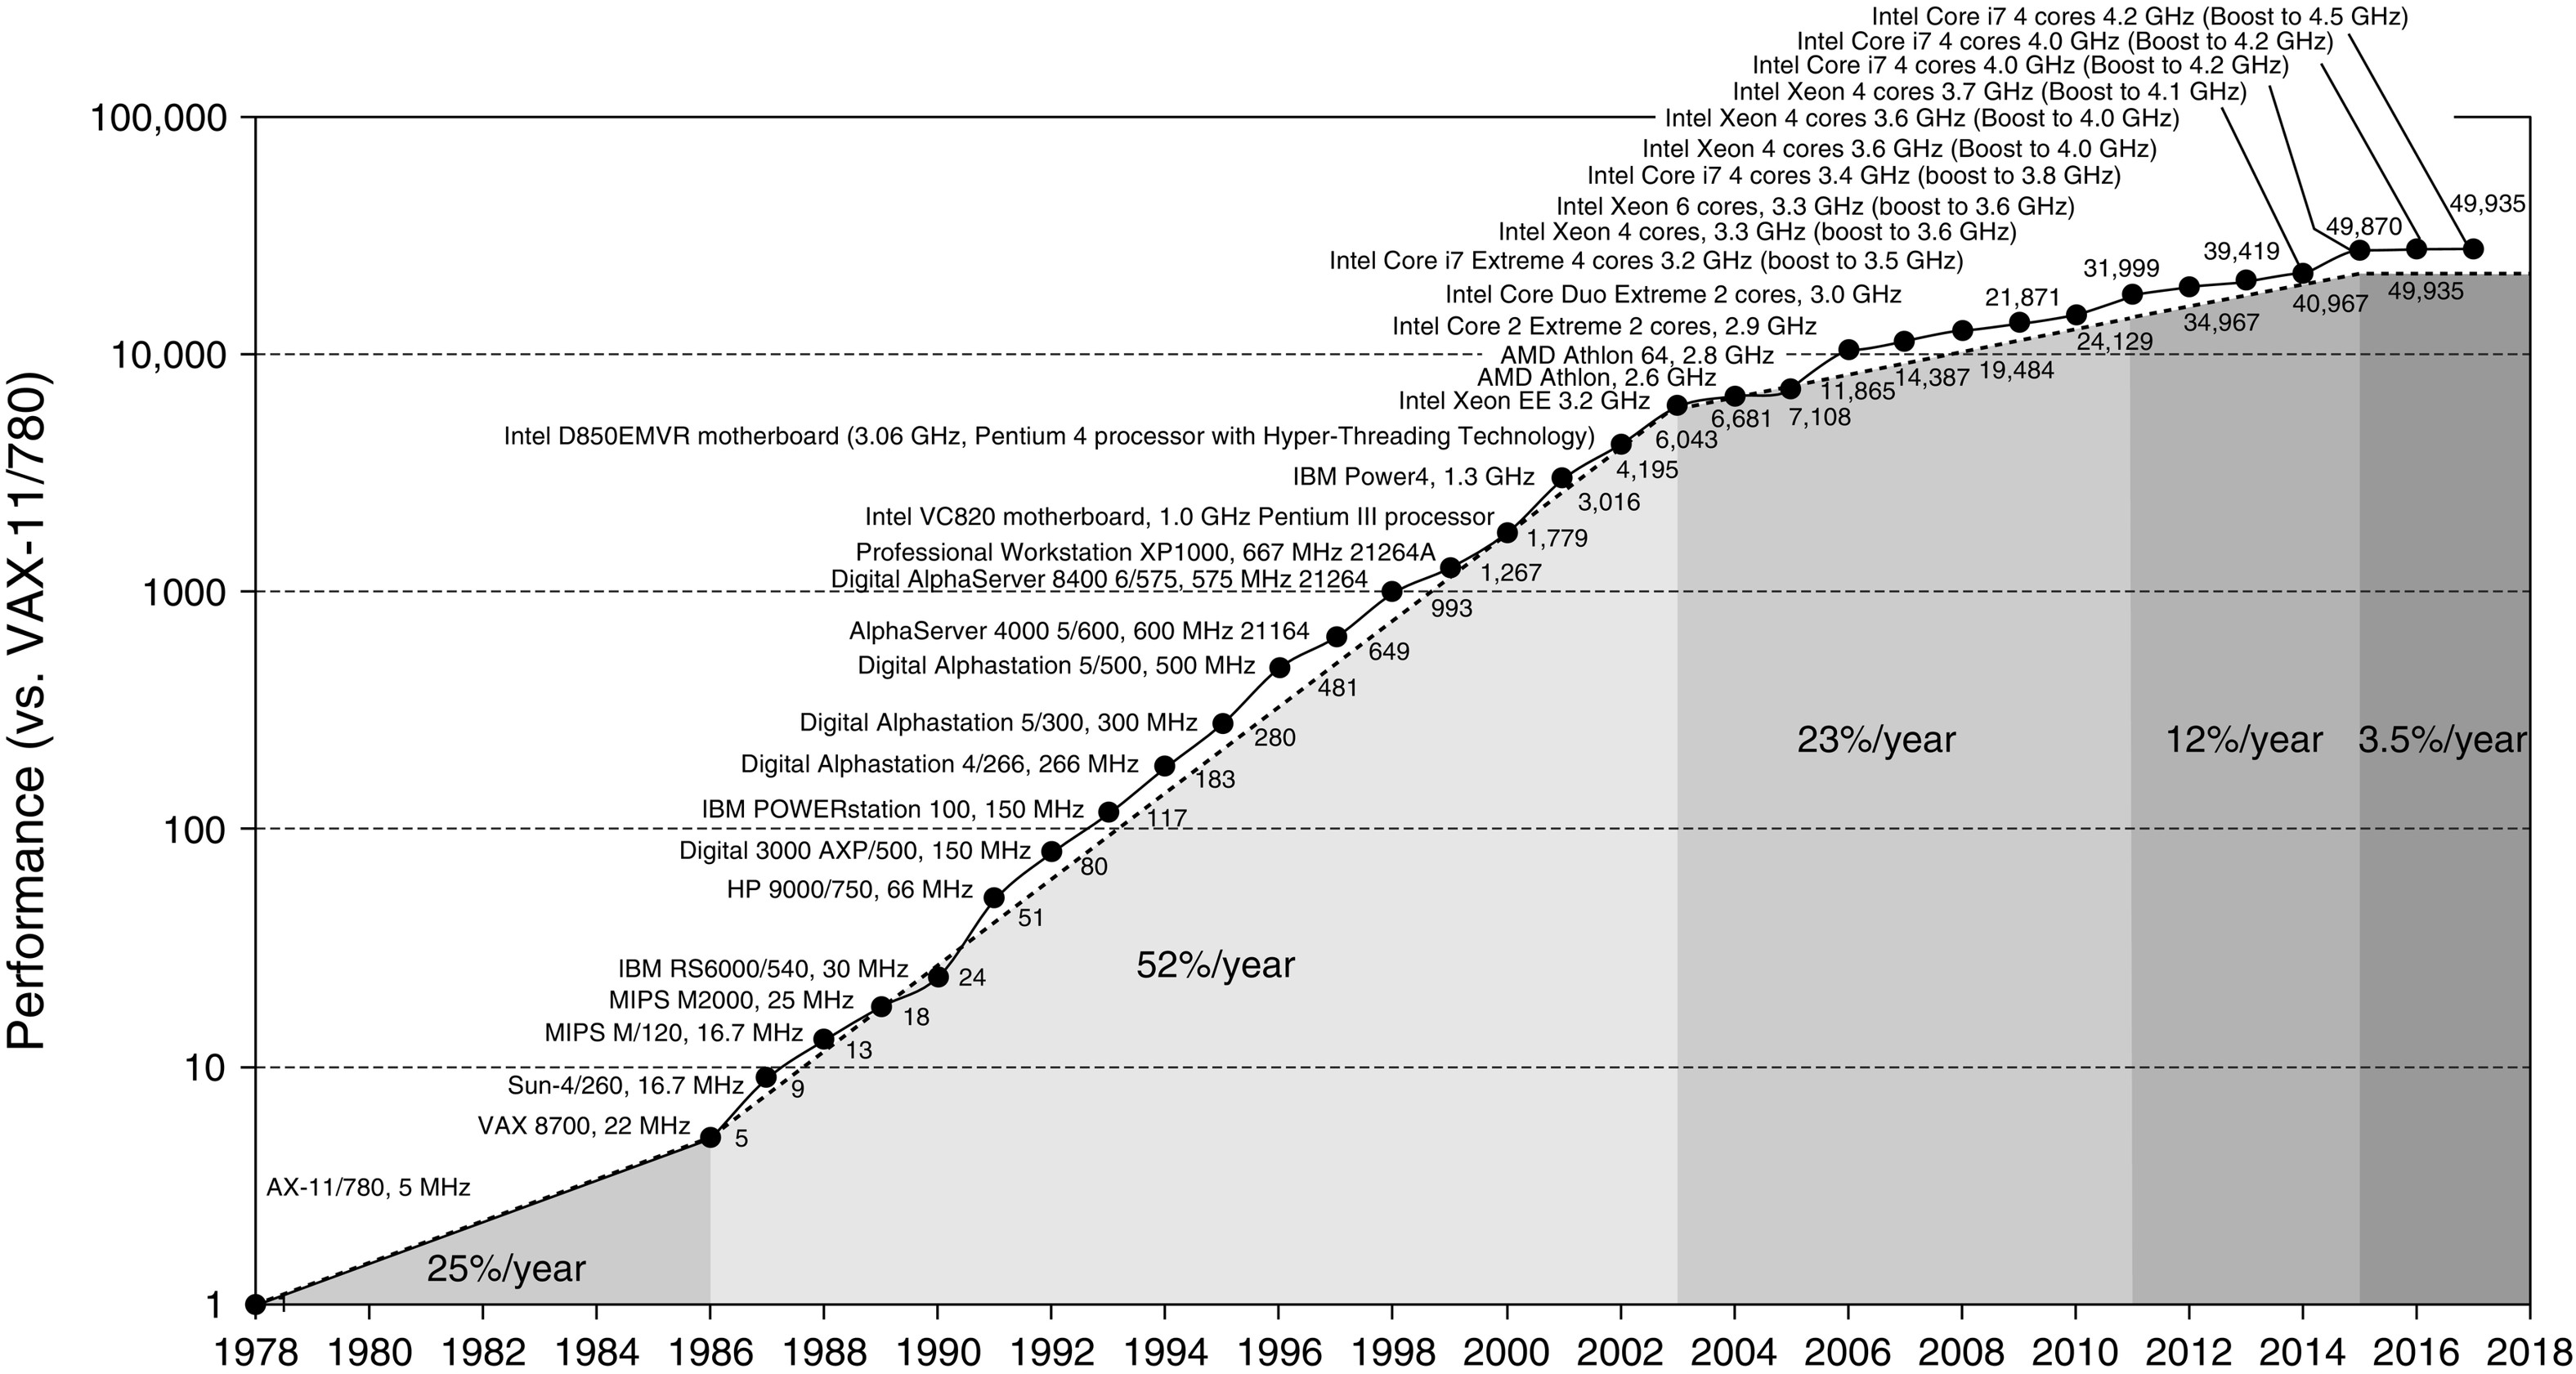
\includegraphics[width=0.8\textwidth]{../Immagini/Capitolo 1/PrestazioniProcessori}
    \caption{Crescita nelle prestazioni dei processori dal 1978 al 2018; il grafico riporta le prestazioni dei processori disponibili sul mercato relative al VAX11/780 misurate attraverso i \textit{benchmark} SPECint.}
    \label{fig:PrestazioniProcessori}
    \par\small{\textit{Fonte: J.L. Hennessy, D.A. Patterson, Computer Architecture: A quantitative Approach. Ed. 6. Waltham, MA:Elsevier, 2017}}
\end{figure}
% Paragrafo 1.3: Le sfide nella progettazione di software parallelo
\section{Le sfide nella progettazione di software parallelo}
\label{par1.3}
Una caratteristica fondamentale posseduta da ogni programma a esecuzione parallela
è la scalabilit\'a, ovvero la capacit\'a di un sistema software di incrementare le proprie prestazioni in funzione della potenza di calcolo richiesta in un preciso istante \cite{Michael2007},
che consente di ottenere architetture tolleranti ai guasti assieme a un'elevata disponibilit\'a del sistema.

% Parte Finale della tesi
\backmatter

%Bibliografia
\bibliographystyle{IEEEtrans}
\addcontentsline{toc}{chapter}{Bibliografia}
\bibliography{./Bibliografia/Bibliografia.bib}

\end{document}